\documentclass[a4paper,12pt]{article}
\usepackage[czech]{babel}
\usepackage[utf8]{inputenc}
\usepackage[FM, noheader]{tul}
\usepackage[unicode]{hyperref}
\usepackage{graphicx}
\usepackage{subcaption}
\usepackage{amsfonts}
\usepackage{indentfirst}

\title{MTLB_cv6}
\author{Petr Boháč}
\date{\today}

\TULphone{+420\,485\,35\,3037}
\TULmail{petr.bohac@tul.cz}

\begin{document}

\section*{MATLB cv. 6 - Analýza funkcí}

    
    Funkce:
    
    \begin{equation}
        f(x) = tan^{-1} \frac{x+1}{x-1}
    \end{equation}
    \begin{equation}
        g(x) = \frac{x}{\sqrt{x^2-1}}
    \end{equation}
    \begin{equation}
        h(x) = x^x
    \end{equation}


    Definiční obory:
    
    \begin{itemize}
        \item $D f(x) = \mathbb{R} \setminus{\{1\}} $
        \item $D g(x) = (-\infty; -1) \cup (1; \infty) $
        \item $D h(x) = (0; \infty), x \in \mathbb{R} $
    \end{itemize}
    
    Limity:
    
    \begin{table}[h]
        \centering
        \caption{Hodnoty funkcí v limitních bodech}
        \begin{tabular}{c|c|c|c}
           Limita & $f(x)$ & $g(x)$ & $h(x)$ \\
           \hline
           $\lim_{x\to\infty}$ & $\frac{\pi}{4}$ & 1 & $\infty$ \\
           $\lim_{x\to-\infty}$ & $\frac{\pi}{4}$ & -1 & 0 \\
           $\lim_{x\to1^{+}}$ & $\frac{\pi}{2}$ & $\infty$ & 1 \\
           $\lim_{x\to1^{-}}$ & $\frac{-\pi}{2}$ & $\sqrt{-\infty}$ & 1 
        \end{tabular}
        \label{tab:my_label}
    \end{table}
    
    
    Grafy funkcí:
    
    \begin{figure}[hb]
        \centering
        \begin{subfigure}{.33\textwidth}
          \centering
          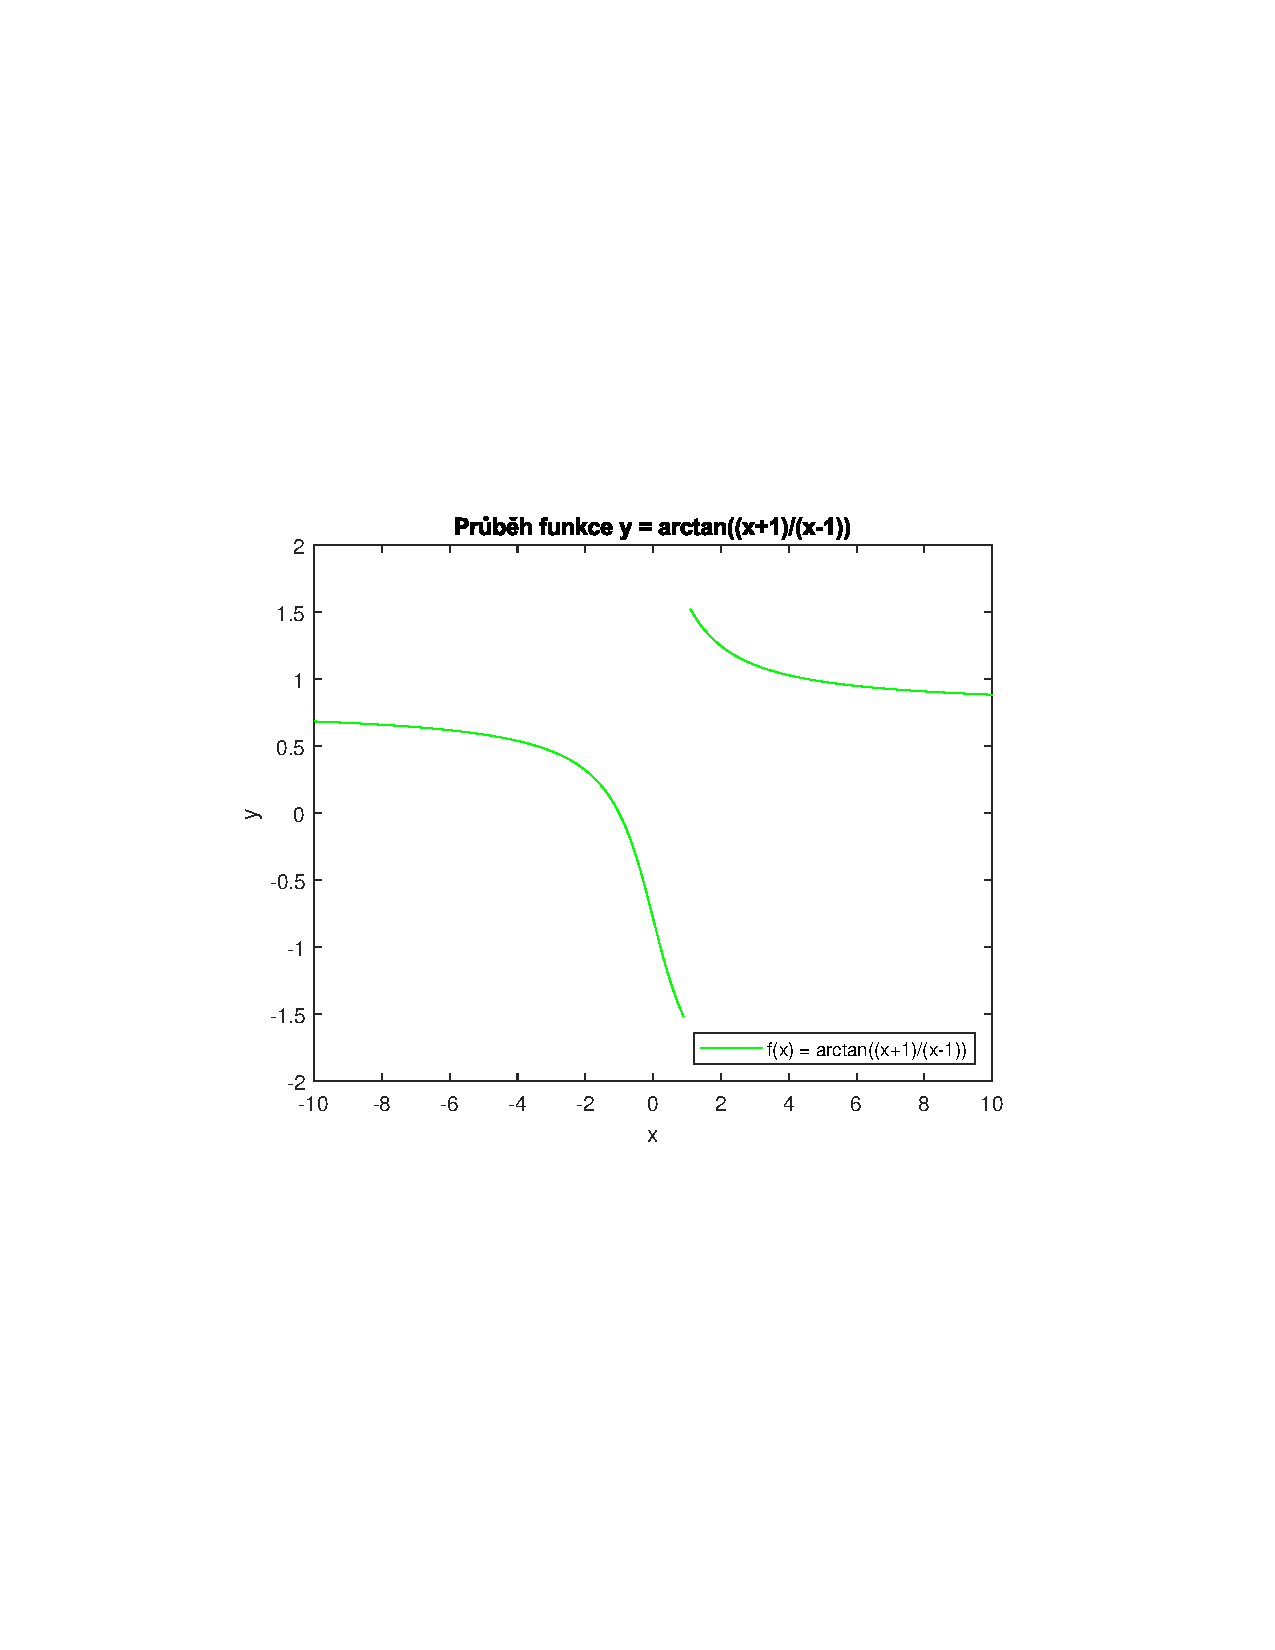
\includegraphics[width=.9\linewidth]{fx.pdf}
          \caption{$f(x)$}
          \label{fig:sfig1}
        \end{subfigure}%
        \begin{subfigure}{.33\textwidth}
          \centering
          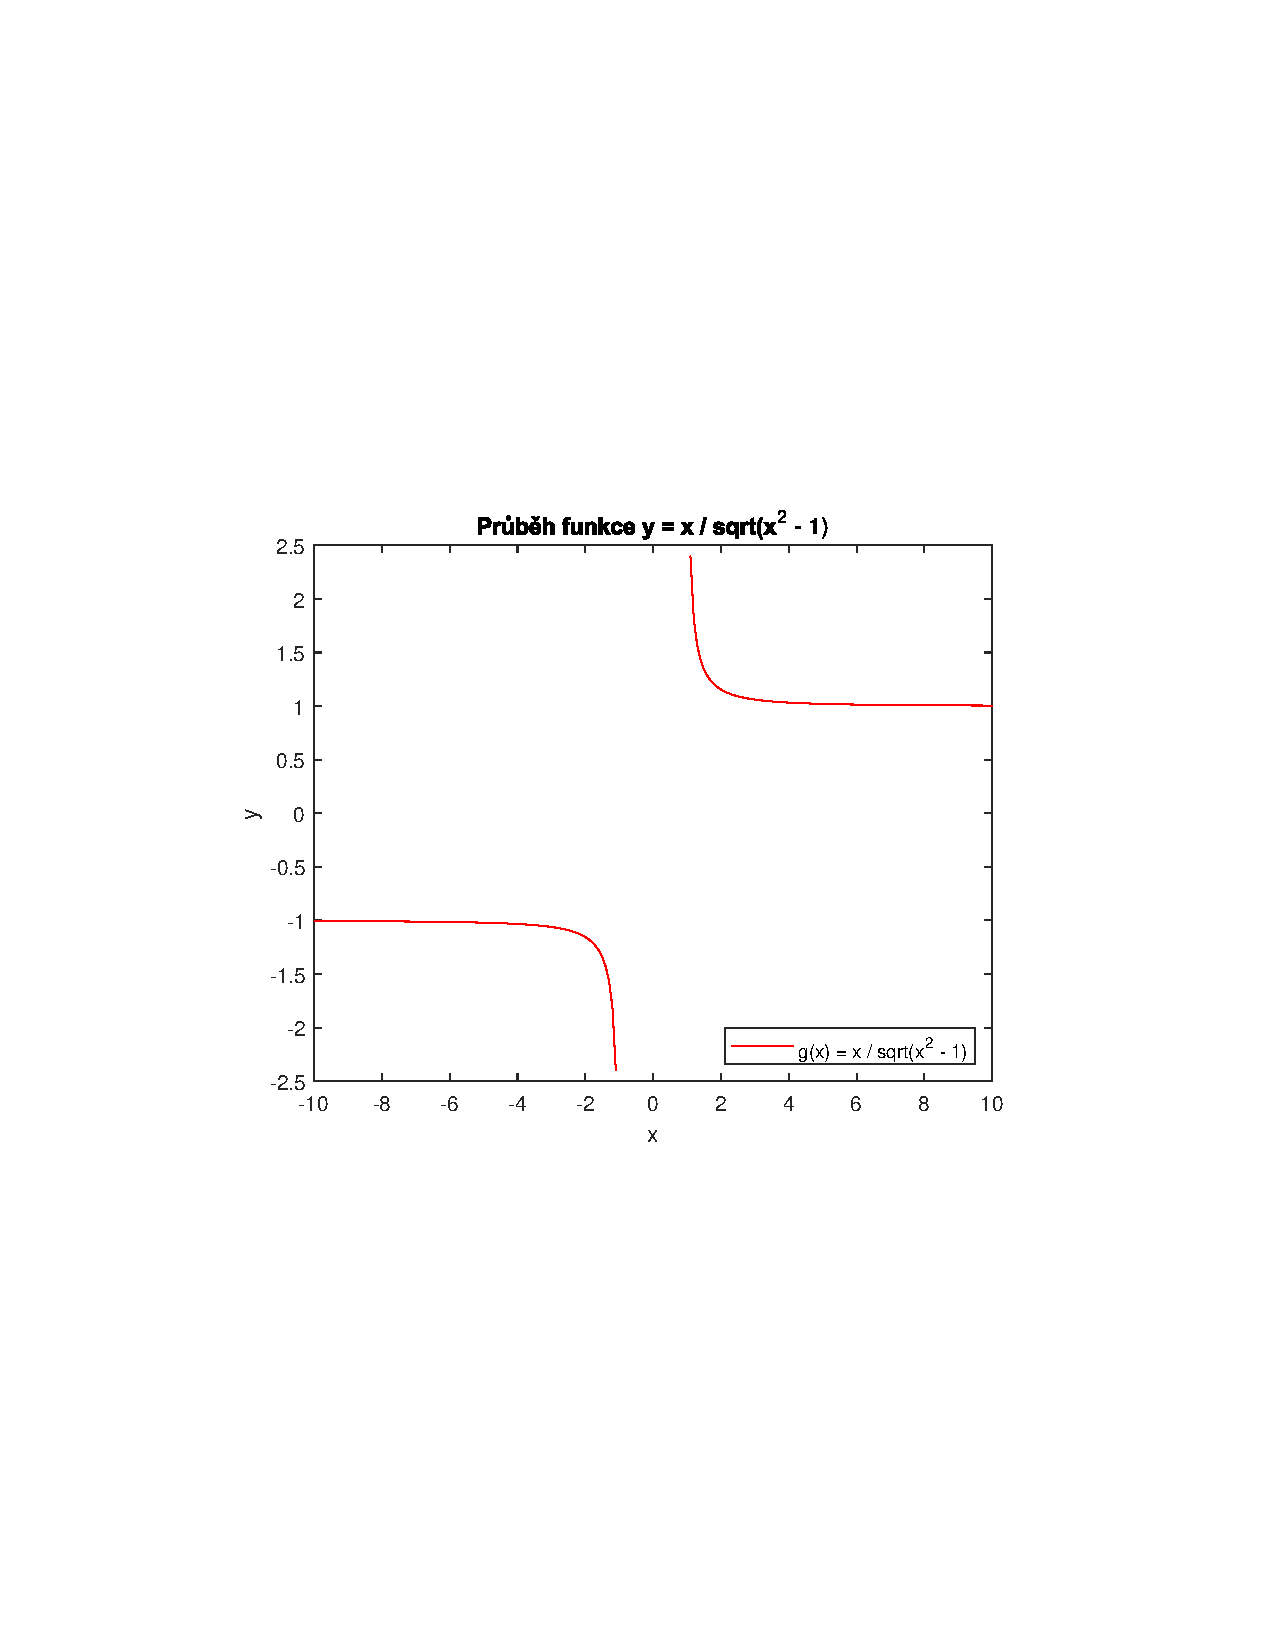
\includegraphics[width=.9\linewidth]{gx.pdf}
          \caption{$g(x)$}
          \label{fig:sfig2}
        \end{subfigure}%
        \begin{subfigure}{.33\textwidth}
          \centering
          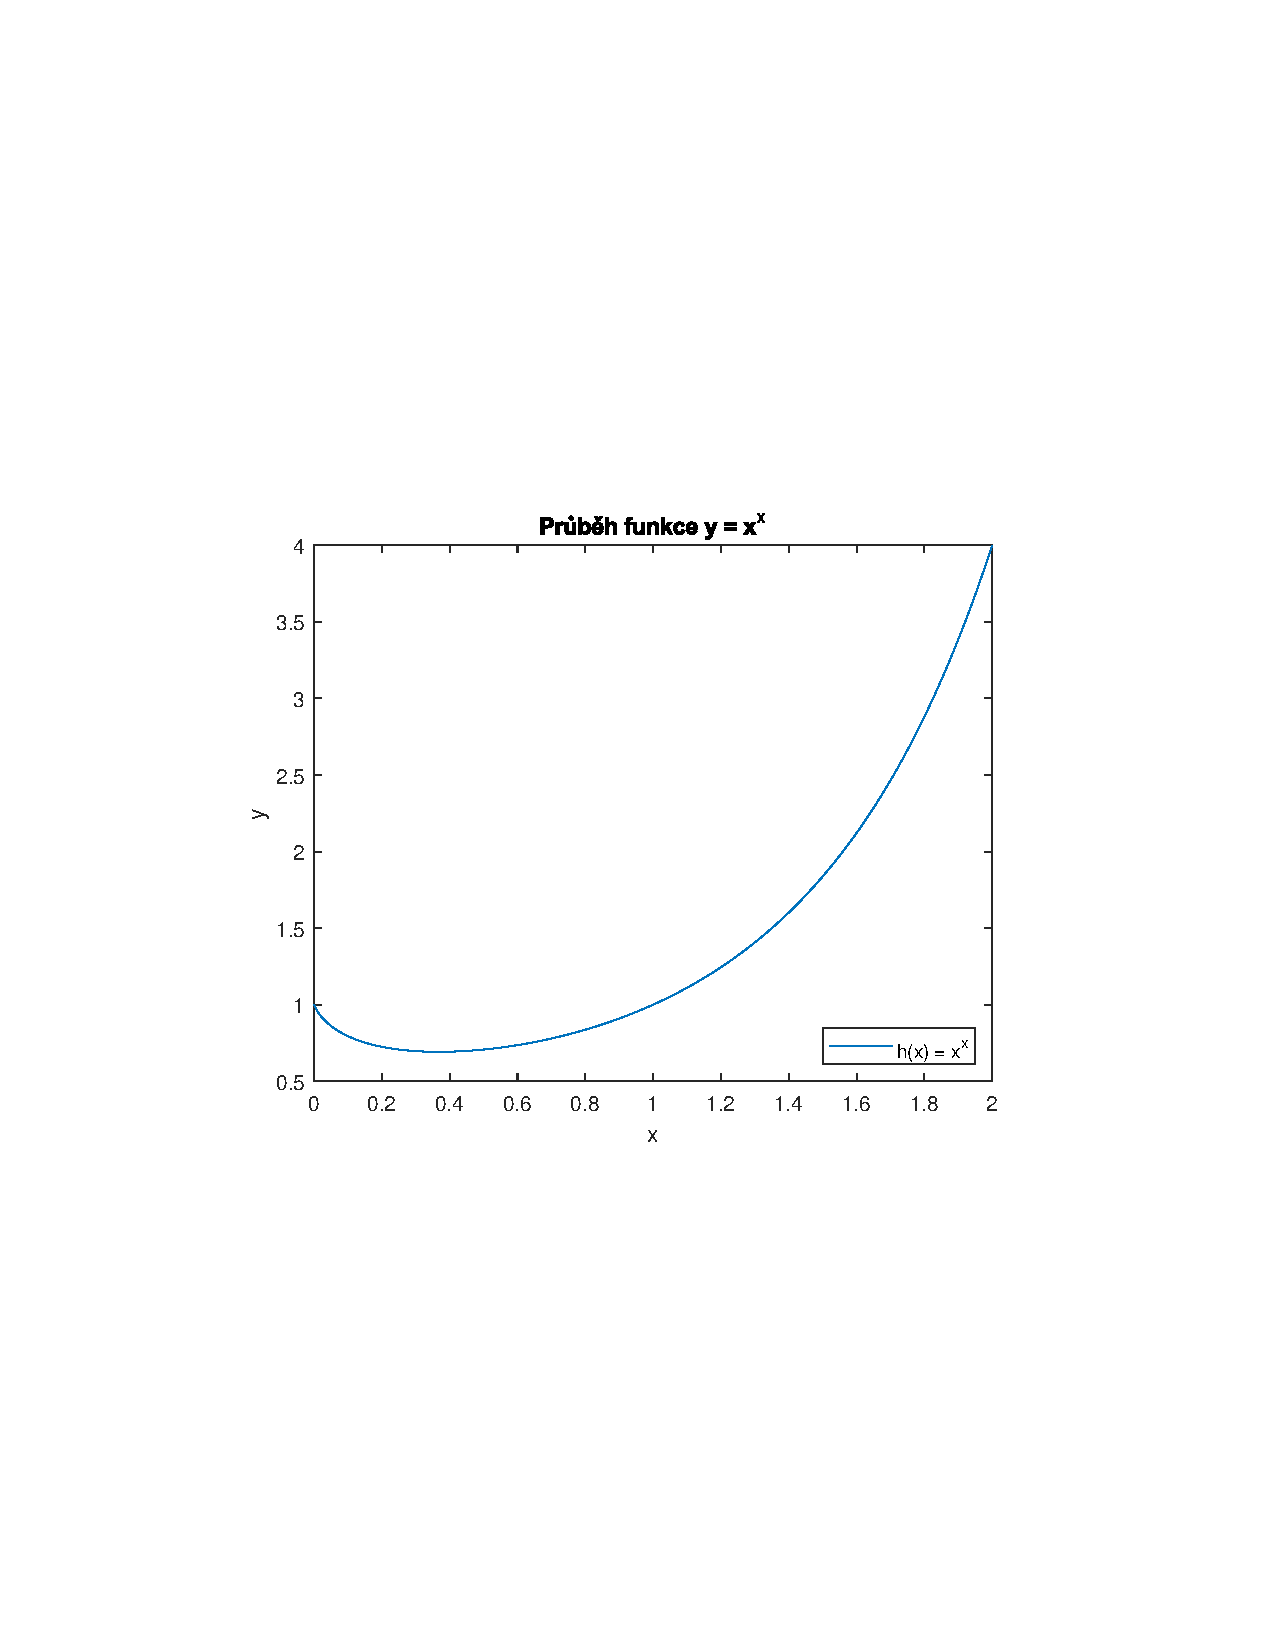
\includegraphics[width=.9\linewidth]{hx.pdf}
          \caption{$h(x)$}
          \label{fig:sfig3}
        \end{subfigure}%
        \caption{Průběh analyzovaných funkcí}
        \label{fig:figs}
    \end{figure}
    
        



\end{document}